% !TEX program = pdflatex
\documentclass[pdftex]{article}
\usepackage{iclr2025_conference,times}
\usepackage{booktabs}
\usepackage{multirow}
\usepackage{amsmath}
\usepackage{amsfonts}
\usepackage{bm}
\usepackage{hyperref}
\usepackage{url}
\usepackage{graphicx} % 加载图形包
\usepackage{caption} % 导入caption包以自定义caption格式
\usepackage{cleveref}
\usepackage{algorithm}
\usepackage{algorithmicx}  
\usepackage{algpseudocode}
\usepackage{verbatim}
\usepackage{graphicx}  % For \scalebox
\usepackage{subfig}    % For \subfloat
\usepackage{booktabs}  % For \toprule, \midrule, \bottomrule
\usepackage{placeins}
\usepackage{enumitem}
\usepackage{wrapfig}
\usepackage{array}
\newcommand{\ie}{i.e., }


\title{Masked Temporal Interpolation Diffusion for Procedure Planning in Instructional Videos}

% Authors must not appear in the submitted version. They should be hidden
% as long as the \iclrfinalcopy macro remains commented out below.
% Non-anonymous submissions will be rejected without review.

\author{
    \quad \quad \quad \quad  Yufan Zhou$^1$ \quad Zhaobo Qi$^1$ \quad Lingshuai Lin$^1$ \quad Junqi Jing$^1$ \\ 
    \quad \quad \quad \quad  Tingting Chai$^1$ \quad Beichen Zhang$^1$ \quad Shuhui Wang$^1$ \quad Weigang Zhang$^1$\thanks{Corresponding Author.}
    \\
    \quad \quad \quad \quad \quad  $^1$Harbin Institute of Technology 
}


% The \author macro works with any number of authors. There are two commands
% used to separate the names and addresses of multiple authors: \And and \AND.
%
% Using \And between authors leaves it to \LaTeX{} to determine where to break
% the lines. Using \AND forces a linebreak at that point. So, if \LaTeX{}
% puts 3 of 4 authors names on the first line, and the last on the second
% line, try using \AND instead of \And before the third author name.
\newcommand{\fix}{\marginpar{FIX}}
\newcommand{\new}{\marginpar{NEW}}

% \iclrfinalcopy % Uncomment for camera-ready version, but NOT for submission.
\begin{document}

\maketitle
\begin{abstract}
In this paper, we address the challenge of procedure planning in instructional videos, aiming to generate coherent and task-aligned action sequences from start and end visual observations. 
% pre
Previous work has mainly relied on text-level supervision to bridge the gap between observed states and unobserved actions, but it struggles with capturing intricate temporal relationships among actions. 
% propose
Building on these efforts, we propose the Masked Temporal Interpolation Diffusion (MTID) model that introduces a latent space temporal logical interpolation module within the diffusion model. 
% module
This module leverages a learnable interpolation matrix to generate intermediate latent features, thereby augmenting visual supervision with richer mid-state details. By integrating this enriched supervision into the model, we enable end-to-end training tailored to task-specific requirements, significantly enhancing the model's capacity to predict temporally coherent action sequences. 
Additionally, we introduce an action-aware mask projection mechanism to restrict the action generation space, combined with a task-adaptive masked proximity loss to prioritize more accurate reasoning results close to the given start and end states over those in intermediate steps. Simultaneously, it filters out task-irrelevant action predictions, leading to contextually aware action sequences.
% exp
Experimental results across three widely used benchmark datasets demonstrate that our MTID achieves promising action planning performance on most metrics. The code is available at \href{https://anonymous.4open.science/r/MTID-E2E3/README.md}{https://anonymous.4open.science/r/MTID-E2E3/README.md}.
\end{abstract}

\section{Introduction}

Recently, procedure planning has exhibited critical reasoning capability for solving real-world challenges in complex domains, such as robotic navigation~\citep{sermanet2024robovqa,bhaskara2024trajectory} and autonomous driving~\citep{wang2024driving,liao2024bat}. 
Among them, procedure planning in instructional videos~\citep{zhao2022p3iv,wang2023pdpp,li2023skip} has been widely concerned because of its wide application scenarios, which involve identifying and generating coherent action sequences that align with the task's objectives, given the start and end visual observations.

% 说明各个方法的核心
In the field of procedure planning in instructional videos, the primary challenge lies in modeling the temporal evolution mechanism among actions and identifying pertinent conditions that can effectively steer the generation of intermediary actions in scenarios where information is scarce. 
As depicted in \Cref{fig:task}(a), many scholars have resorted to capturing different forms of auxiliary information about the intermediate states to bridge the gap between observed states and unobserved actions. 
% example
For example, event-based supervision~\citep{wang2023event} leverages key task events to help the model learn temporal action structures, while task label supervision~\citep{wang2023pdpp} uses task-specific labels for better alignment with the task objective. The probabilistic procedure knowledge graph~\citep{nagasinghe2024not} provides structured knowledge to enhance the understanding of action dependencies. Additionally, \citet{niu2024schema} leverage large language models (LLMs) to describe state changes, improving the model’s grasp of causal relationships by combining visual and language descriptions.
% problem
%However, these methods rely on text-level supervision instead of visual-level feature supervision, leading to less detailed and comprehensive information. 
However, all these methods are limited to providing text-level supervision, resulting in less detailed and comprehensive information, and failing to precisely capture the temporal relationships between actions. 
Additionally, these methods decouple the acquisition of supervisory information from the intermediate action reasoning process, hindering effective collaboration and interaction between the two. Consequently, it becomes challenging to fully integrate and adapt to current action reasoning tasks. 

%In light of these discrepancies, we investigate reconstructing and complementing the mid-state visual supervision by computing the temporal logical relationships between actions.

\begin{figure}[t]
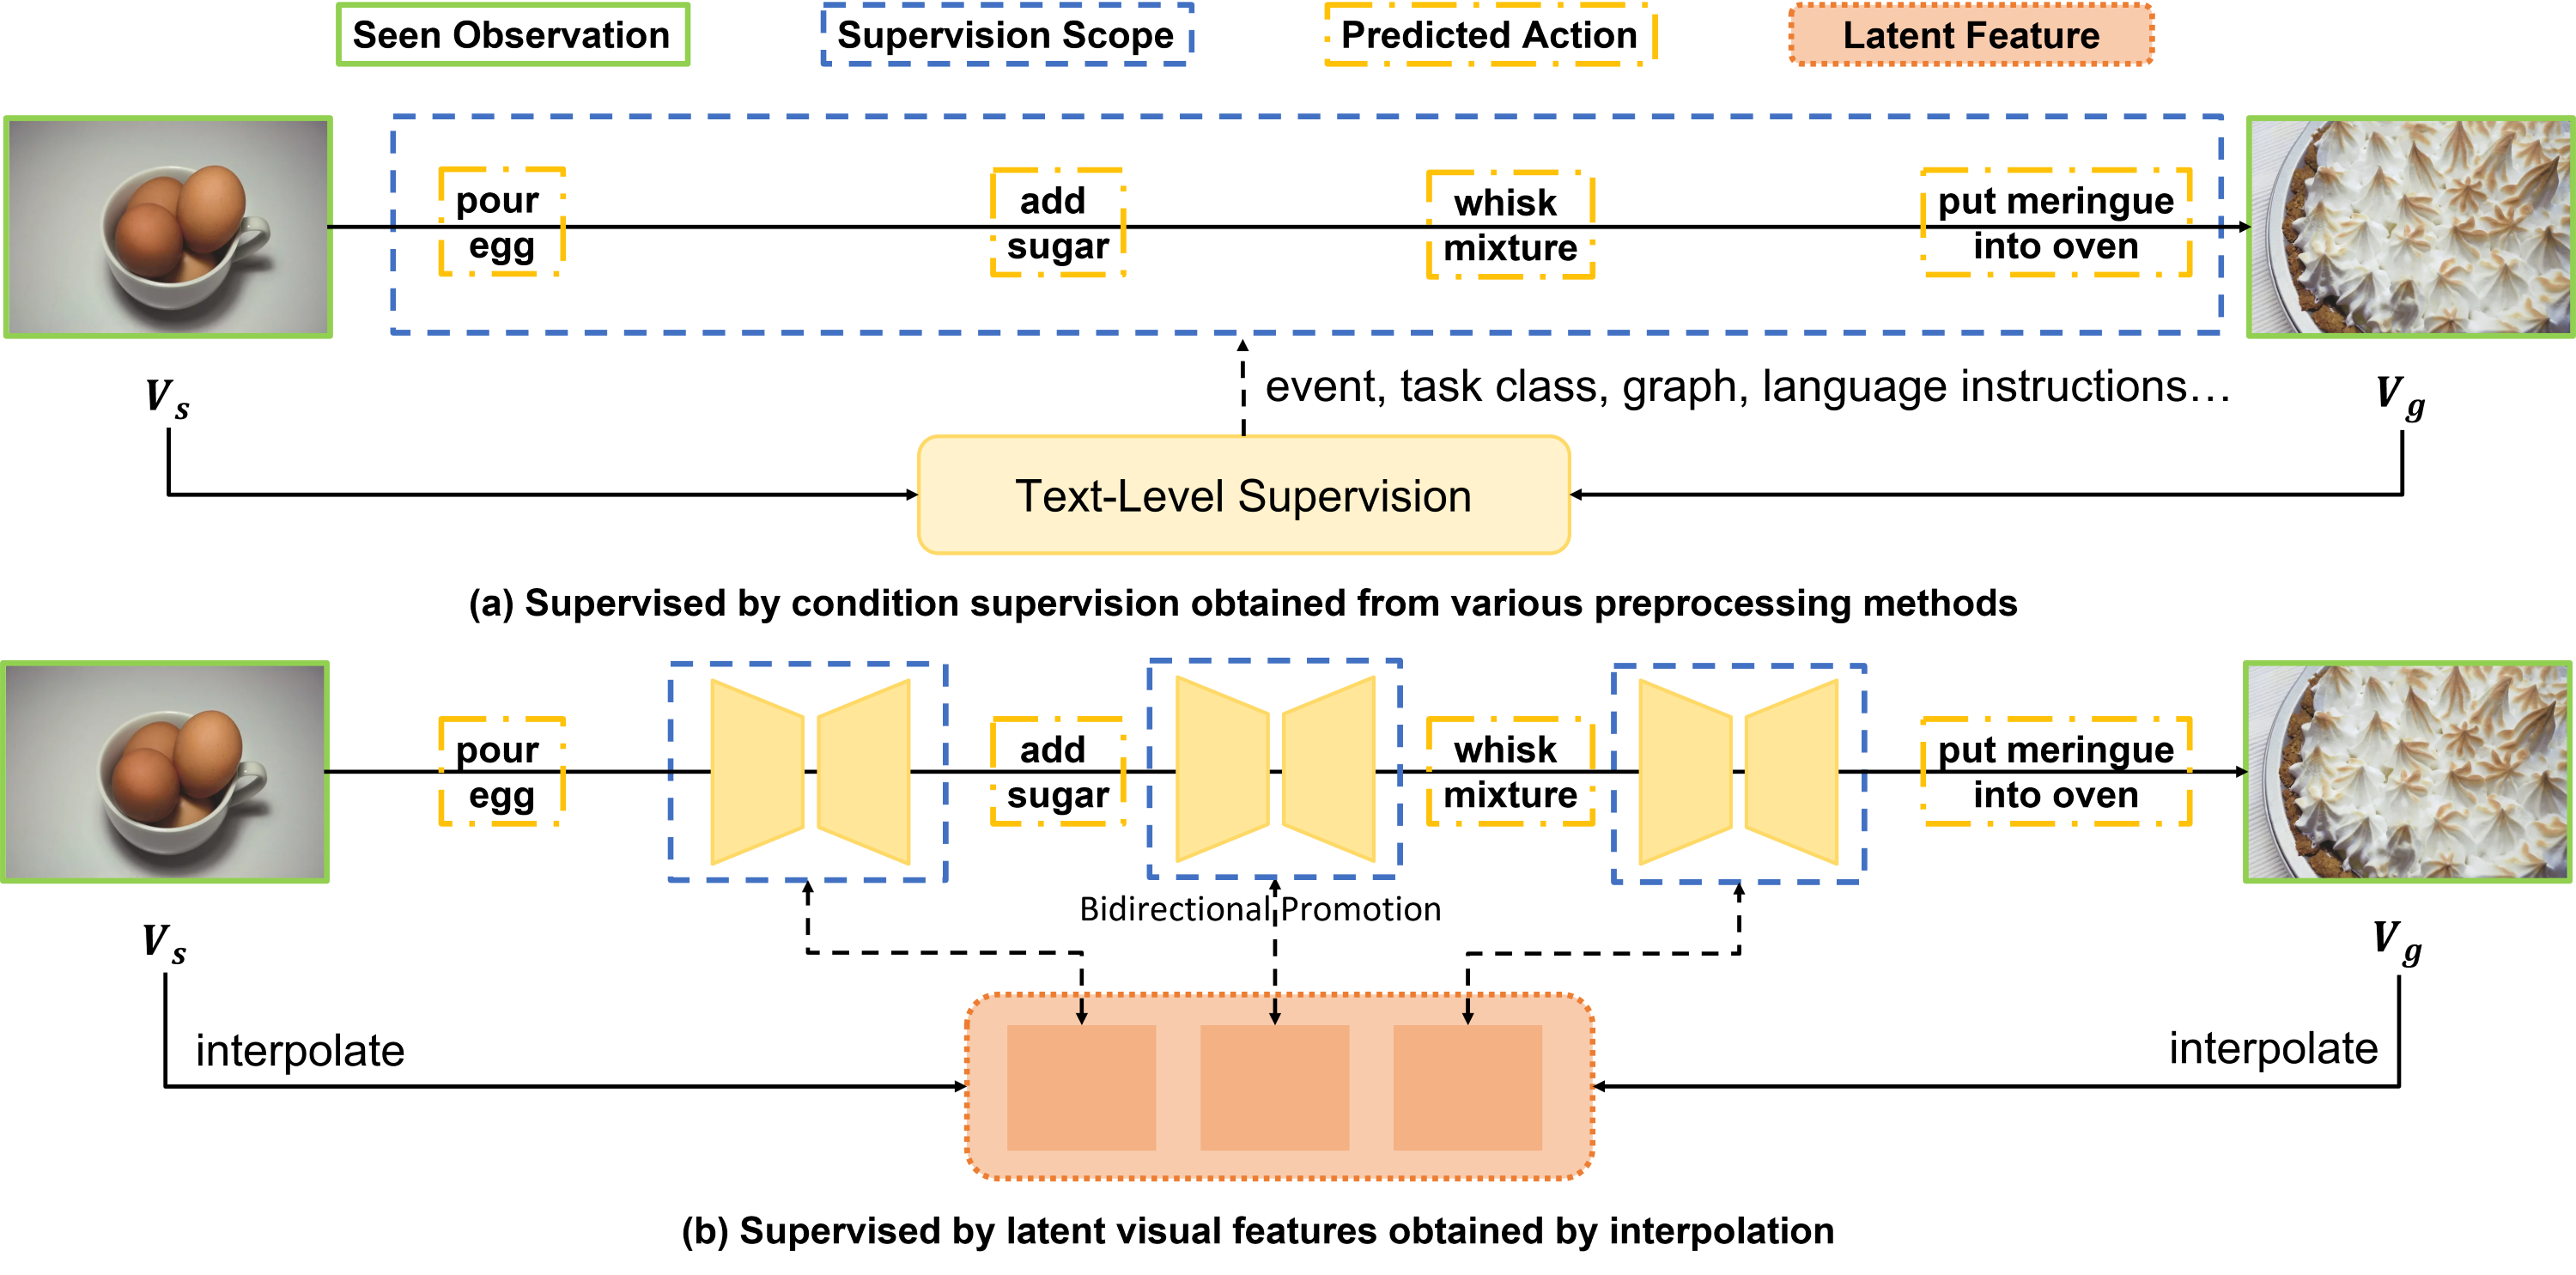
\includegraphics[width=0.98\textwidth, keepaspectratio]{figures/fig-task.png}
% \vspace{-0.5em}
\caption{The core idea to solve procedure planning with previous methods and ours. }
\label{fig:task}
% \vspace{-2.5mm}
\end{figure}

%%%%%%%%%%%
% 这个是一个总括,波波倒数第二段
%%%%%%%%%%%%
Based on the above analysis, we propose the Masked Temporal Interpolation Diffusion (MTID) model for procedure planning in instructional videos. 
As shown in \Cref{fig:task}(b), the core concept is to leverage intermediate latent visual features, generated synchronously by a latent space temporal logical interpolation module, to provide comprehensive visual-level information for mid-state supervision. 
In the meanwhile, the generated visual features are directly injected into the action reasoning model, ensuring the generation of intermediate supervision information can be effectively applied to the current action reasoning task through end-to-end training.

%%%%%%%%%%%%%%
% 总结我们的主要贡献
%%%%%%%%%%%
% 构成
Specifically, \textbf{MTID} consists of three core components: a task classifier, a latent space temporal logical interpolation module, and a diffusion model framework that incorporates both a U-Net and a DDIM strategy.
% first
In the first stage, a transformer-based classifier predicts the task class label $c$ for the entire instructional video, given the start and end observations. This prediction serves as the foundation for subsequent reasoning and action generation.
% second
The latent space temporal logical interpolation module is designed to capture and model temporal relationships. 
% 1
It employs an observation encoder to transform the visual features of the observations into latent features that maintain temporal dependencies and discard object details. 
% 2
A latent space interpolator then generates intermediate features using a learnable interpolation matrix, which dynamically adjusts the interpolation ratio to fit task-specific requirements. 
% 3
These interpolated features are refined through transformer blocks, enhancing their temporal coherence and capturing the dependencies between action sequences.
% third
In the third stage, during the denoising phase for generating action sequences, the input matrix is constructed by concatenating the task class label, observed visual features, and Gaussian noise sampled from $\mathcal{N}(0, I)$. 
% mask
A masked projection is applied to exclude irrelevant actions, ensuring that the generated actions remain within the desired range. 
% ddim
To accelerate inference, DDIM is used throughout the iterative process.
% loss
To further ensure task relevance, a task-adaptive masked proximity loss is introduced. This loss function gradually decreases its focus toward the central features, reinforcing supervision on intermediate latent features while penalizing irrelevant actions, thereby constraining the generation process. 
% all
By leveraging detailed information from both the start and end observations $V_s$ and $V_g$, our model accurately predicts target action sequences, as demonstrated by experimental results on the CrossTask, COIN, and NIV datasets.

The main contributions of this paper are as follows:
\begin{itemize}[leftmargin=*]
%\vspace{-2mm}
    \item We propose a Masked Temporal Interpolation Diffusion model with a mask to limit action initialization and a task-adaptive masked proximity loss to enhance accuracy.
    
    \item We use a latent space temporal logical interpolation module to extract intermediate visual features with temporal relationships from the start and end states to guide the diffusion process.
    
    \item Extensive experiments are conducted on several widely used benchmarks, showing significant performance improvements on multiple tasks using the proposed method.
\end{itemize}




% Specifically, \textbf{MTID} consists of a transformer-based classifier, a latent space temporal logical interpolation module, and a diffusion model framework, which includes a U-Net and a DDIM strategy. Given a start observation $V_s$ and a goal observation $V_g$, the transformer-based classifier assigns the corresponding task labels $c$ for task supervision. For the latent space temporal logical interpolation module, the observation encoder $E$ transforms the input observations $V_s$ and $V_g$ into latent features $L_s$ and $L_g$, converting the visual features with object details into logical features with temporal relationships. The interpolator then generates intermediate latent features $I_{1:M}$ by applying a learned interpolation matrix $\phi$, dynamically adjusting the interpolation ratio to adapt to different tasks. These latent features are further refined through transformer encoder blocks $TF$, producing intermediate features $F_{1:M}$, with additional temporal logical information. Next, concatenating noise $\varepsilon_{1:T} \sim \mathcal{N}(0, I)$, the task label $c$, and the observations $V_s$ and $V_g$ into the matrix $\hat{x}_N$, we apply a masked projection to $\hat{a}_{1:T}$ during initialization to restrict irrelevant actions during iteration. This is then input into the U-Net model $f_\theta$ to fit the distribution of the target actions $a_{1:T}$. During this process, $F_{1:M}$ is incorporated via cross-attention to assist in the fitting. A task-adaptive masked proximity loss $\mathcal{L}_{\mathrm{diff}}$ is also applied to strengthen supervision of the intermediate latent features and penalize actions that do not align with the task. Consequently, with the detailed information from $V_s$ and $V_g$, the model can predict target action sequences, as demonstrated across various datasets.

% 太细节化  流程化了   讲了一遍方法的流程  没啥意思
% 讲你那插值   mask和loss的目的  核心思想   好处就行    让人明白最high-level的东西

\section{Related Work}
\label{gen_inst}
\textbf{Procedure Planning in Instructional Videos.} focuses on making goal-directed plans given the current visual observations in unstructured real-life videos. 
In this work, we follow formulation of PDPP~\citep{wang2023pdpp}  of procedure planning. 
Early work framed the task as sequential latent space~\citep{chang2020procedure} and used adversarial policy learning~\citep{bi2021procedure}. 
Several methods have been proposed to enhance planning, such as replacing visual states with linguistic supervision to predict steps~\citep{zhao2022p3iv}, modeling action sequence distribution using diffusion models~\citep{wang2023pdpp}, applying mask-and-predict strategies to mine step relationships~\citep{wang2023event}, and breaking sequences into shorter sub-chains by skipping unreliable actions~\citep{li2023skip}. 
Recently, KEPP~\citep{nagasinghe2024not} similarly integrates probabilistic procedural knowledge for complex step sequencing. And SCHEMA~\citep{niu2024schema} focuses on tracking state changes at each step. 
Our approach builds on these, aiming for more efficient, accurate planning by utilizing the calculated temporal logical relationships. 

\textbf{Diffusion Probabilistic Models for Long Video Generation.} Recent advancements in diffusion probabilistic models~\citep{croitoru2023diffusion} , initially popularized in image generation~\citep{rombach2022high}, have shown promising results in generating high-quality long video sequences~\citep{weng2024art,zhou2024upscale,jiang2024videobooth}. For example, StreamingT2V~\citep{henschel2024streamingt2v} enables the creation of temporally consistent long videos with smooth transitions and high frame-level image quality, extending beyond typical short video generation limitations. StoryDiffusion~\citep{zhou2024storydiffusion}, a method incorporating Consistent Self-Attention to enhance coherence in generated sequences of images or videos, allows for the creation of visually consistent stories with rich detail. These advancements address challenges like maintaining temporal coherence and generating realistic motion in longer video sequences. 
\section{Method}
\subsection{Overview}
\label{method1}

Following \citet{chang2020procedure}, given an initial visual observation $V_s$ and a target visual observation $V_g$, both are short video clips indicating different states of the real-world environment extracted from an instructional video, the procedure planning task aims to generate a sequence of actions $a_{1:T}$ that transforms the environment from $V_s$ to $V_g$, where $T$ denotes the number of planning time steps. This problem can be formulated as $p(a_{1:T} \mid V_s, V_g)$. 

Considering the weak temporal reasoning ability caused by the absence of intermediate visual states, especially in long video scenarios, we propose the \textbf{Masked Temporal Interpolation Diffusion} (MTID) framework, which employs a denoising diffusion model to rapidly predict the intermediate action sequence $a_{1:T}$. As outlined in the following formula, MTID decomposes the procedure planning task into three sub-problems, 
\begin{equation} 
    p(a_{1:T} \mid V_{s}, V_{g}) = \iint p(a_{1:T} \mid \upsilon_{1:M}, c, V_{s}, V_{g}) p(\upsilon_{1:M} \mid V_{s}, V_{g}) p(c \mid V_{s}, V_{g}) d\upsilon_{1:M} dc .
    \label{eq:1}
\end{equation}
The first sub-problem entails capturing information about the task to be completed about the whole instructional video, serving as the basis for subsequent reasoning. 
As shown in~\Cref{fig:architecture}, this task supervision stage solves a standard classification problem using a transformer encoder to extract features from observation pair $\left\{ {V_s, V_g} \right\}$ and transform them into task class label $c$.

The second sub-problem focuses on reconstructing $M$ intermediate visual features $\upsilon_{1:M}$ from $V_s$ and $V_g$ to address the lack of mid-state visual supervision and reveal hidden temporal logic within the action sequences, which is achieved through our latent space temporal logical interpolation module. 

The final sub-problem involves generating action sequence $a_{1:T}$ based on the task information and interpolated intermediate features. 
Specifically, we first construct the input matrix $\hat{x}_N$ for the denoising steps, which consists of three dimensions. 
The task class dimension contains the captured task information $c$ for each reasoning step.
The observation dimension contains the visual observations of the start and goal states $\left\{ {V_s, V_g} \right\}$, where the intermediate states are set to zero. 
The action dimension $\hat{a}_{1:T}$ represents the target intermediate action sequence, which is initialized by $\epsilon \sim \mathcal{N}(0, I)$ and further constrained by our action mask mechanism to reduce the action space to be predicted.
Hence, the iteration matrix $\hat{x}_n \in \mathbb{R}^{ T \times (C+A+O)  }$ is expressed as, 
\begin{equation}
    \hat{x}_n = \begin{bmatrix}  
        c & c & \cdots & c & c \\  
        \hat{a}_1 & \hat{a}_2 & \cdots & \hat{a}_{T-1} & \hat{a}_T \\  
        V_s & 0 & \cdots & 0 & V_g
    \end{bmatrix},
\end{equation}
where $n$ ranges from 0 to $N$, $C$ is the number of task classes, $A$ is the number of actions and $O$ is the observation visual feature dimension. Next, the intermediate latent features generated from the latent space temporal logical interpolation module will be injected into the diffusion model to iteratively optimize the matrix $\hat{x}_n$. 
During the iteration process, we adopt DDIM to accelerate the sampling process with fewer steps while maintaining strong performance. 
Lastly, we introduce the task-adaptive masked proximity loss $\mathcal{L}_{\mathrm{diff}}$ to enhance the reliability of the reasoning results.
\begin{figure}[t]
    \centering
    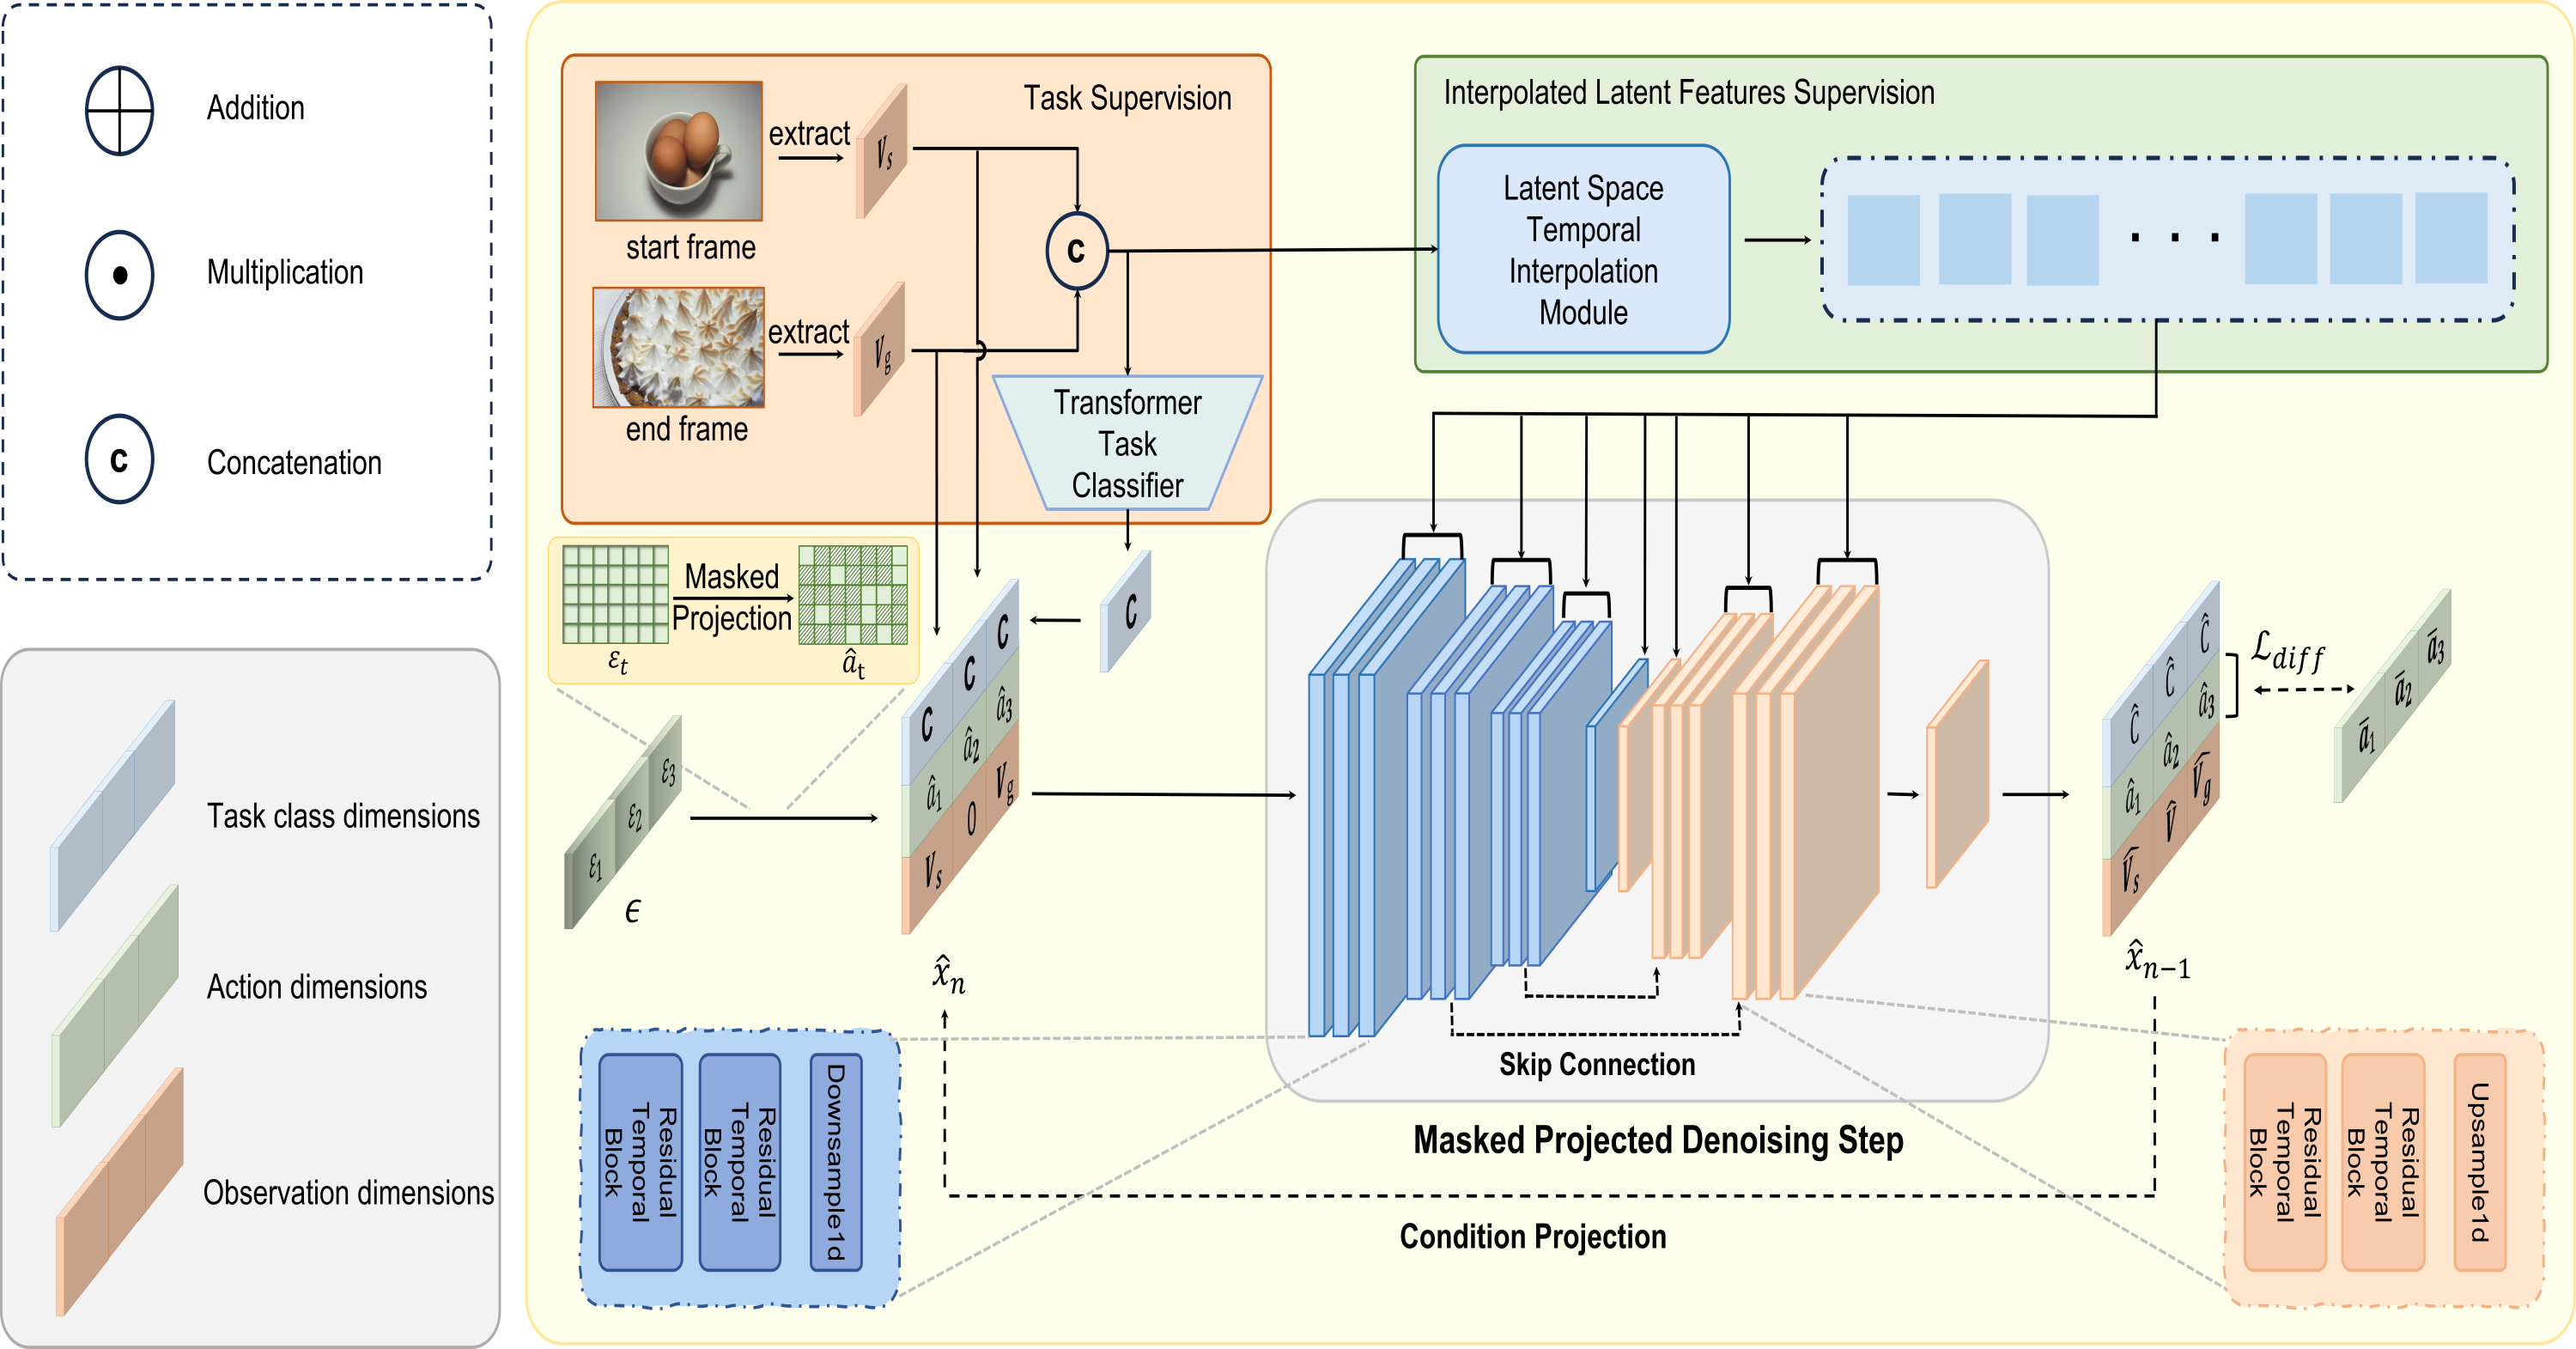
\includegraphics[width=\textwidth,height=0.6\textheight,keepaspectratio]{figures/architecture1.png}
    \caption{Overview of our Masked Temporal Interpolation Diffusion (prediction horizon \( T=3 \)). }
    \label{fig:architecture}
\vspace{-4mm}
\end{figure}
% We first train a transformer task classifier to generate condition information \( c \), which will be used as guidance along with the given observations \( V_s \) and \( V_g \). Subsequently, we put the concatenated observations into the latent space temporal logical interpolation module to obtain the latent temporal logic supervision. Then we compute the denoising process iteratively. In the first step, we conduct a masked projection to the input, then predict the initial distribution by the learned model \( f(\theta) \). We calculate \( \hat{x}_{n-1} \) with the U-Net output \( \hat{x}_0 \). After repeated iterations, we finally select the action dimensions as our result after \( N \) denoising steps.


\subsection{MTID: Masked Temporal Interpolation Diffusion}
\label{method2} 

%\subsubsection{Denoising Diffusion Implicit Models for Training and Inference}

\subsubsection{Preliminaries}
\label{method21}

Denoising Diffusion Implicit Model (DDIM)~\citep{song2020denoising} improves sampling efficiency by making the reverse process deterministic, which reduces stochastic noise and establishes a direct mapping between the initial noise matrix \(\hat{x}_N\) and the final output matrix \(\hat{x}_0\) across $N$ non-Markovian steps. This approach reduces the number of steps needed while preserving sample quality. 

Based on these advantages, we adopt the DDIM sampling strategy with the U-Net model~\citep{ronneberger2015u} for its ability to accelerate sampling with fewer steps while maintaining strong performance. This is especially useful in scenarios where the quality of results remains comparable to that of Denoising Diffusion Probabilistic Model (DDPM)~\citep{ho2020denoising,nichol2021improved}, despite its deterministic approach.

The forward process is parameterized as:
\begin{equation}
\hat{x}_N = \sqrt{\bar{\alpha }_N} \, \hat{x}_0 + \sqrt{1 - \bar{\alpha }_N} \, \epsilon,
\end{equation}
where \(\bar{\alpha }_N = \prod_{s=1}^N \alpha_s\), \( \epsilon \sim \mathcal{N}(0, I)\), and \(\alpha_s = 1 - \beta_s\), which represents the noise schedule controlling the amount of Gaussian noise added at each step \(s\). The forward process starts with the original data \(\hat{x}_0\) and progressively adds noise, resulting in the final noisy matrix \(\hat{x}_N\).

In DDIM, the reverse process is defined as:
\begin{equation}
\hat{x}_{n-1} = \sqrt{\bar{\alpha }_{n-1}} \left( \frac{\hat{x}_{n} - \sqrt{1 - \bar{\alpha }_{n}} f_{\theta}\left(\hat{x}_{n}\right)}{\sqrt{\bar{\alpha }_{n}}} \right) + \sqrt{1 - \bar{\alpha }_{n-1}} \cdot f_{\theta}\left(\hat{x}_{n}\right),
\end{equation}
where \( f_{\theta}\left(\hat{x}_{n}\right) \) is the neural network's prediction of the noise component added to \( \hat{x}_n \). This reverse process reconstructs the original data \(\hat{x}_0\) from \(\hat{x}_N\) by iteratively removing the noise introduced during the forward diffusion process. Unlike DDPM, DDIM's deterministic reverse process improves sampling efficiency by directly mapping the noisy input \(\hat{x}_N\) to the final output \(\hat{x}_0\). This makes DDIM an efficient method for generating or enhancing samples with fewer steps.


\subsubsection{Latent Space Temporal Logical Interpolation}
\label{method23}

\input{figures/architecture2}

%and transformer encoder blocks to refine the features and provide more exact information.

As shown in \Cref{fig:architecture2}, the \textbf{Latent Space Temporal Logical Interpolation Module} consists of three core components: an observation encoder, which transforms observation visual features into latent features; a latent space interpolator, which generates multiple features to fill the intermediate supervision; and transformer encoder blocks, which refine the generated features and enhance the module's ability to model the temporal correlations among action sequences.


Specifically, this module first employs an observation encoder $E$, consisting of convolutional layers, to transform the visual observations $V_s$ and $V_g$ into their respective latent features $L_s$ and $L_g$:
\begin{equation}
    L_s, L_g = E(V_s, V_g).
\end{equation}
In the latent space, we perform linear interpolation between $L_s$ and $L_g$ to generate a sequence of interpolated features \{$I_1, I_2, \dots, I_M$\}. 
Unlike fixed linear interpolation, our method dynamically adjusts the interpolation through the learnable interpolation matrix  $\phi \in \mathbb{R}^{M \times O}$ to facilitate smooth and task-specific transitions. 
This matrix, restricted between 0 and 1, is responsible for weighting the latent features $L_s$ and $L_g$ to generate the intermediate latent features as follows:
\begin{equation}
    \begin{split}
        \phi &= Sigmoid(W \cdot \mathbf{\tau} + k), \\
        I_j &= (1 - \phi_j) \cdot L_s + \phi_j \cdot L_g,
    \end{split}
\end{equation}
where $W \in \mathbb{R}^{M \times O}$ and $k \in \mathbb{R}^{M \times O}$ are the parameters of the linear layer, and $O$ represents the observation dimension. The matrix $\mathbf{\tau} \in \mathbb{R}^{M \times O}$ is a learnable matrix initialized with a constant value, controlling a variable ratio between $L_s$ and $L_g$. This method requires no parameter tuning and offers better adaptability to different tasks. The number of latent features $M$ depends on the number of residual temporal blocks in the model.



The sequence of interpolated features $\{I_1, I_2, \dots, I_M\}$ is then passed through a series of transformer encoder blocks $TF$ to obtain the enhanced latent features:
\begin{equation}
    F_1, F_2, \dots, F_M = TF(I_1, I_2, \dots, I_M).
\end{equation}
The self-attention mechanism in the transformers captures dependencies between latent features at different time steps by computing attention scores across all latent features. Stacking multiple transformer blocks allows the model to iteratively refine these features, ensuring that temporal and contextual relationships are effectively learned.


% With these latent features  containing temporal logical information, 

To integrate the interpolated latent features $\{F_1, F_2, \dots, F_M\}$ into the model during the denoising process, we incorporate cross-attention layers~\citep{khachatryan2023text2video} into the residual temporal blocks of the U-Net, as shown in \Cref{fig:architecture3}. This allows the model to dynamically focus on relevant latent features through a learnable matrix, enhancing its ability to capture complex relationships with more latent temporal logical information and improving the quality of action predictions.

In this setup, the latent feature $F_j$, processed through a linear layer, serves as the key and value, while $\hat{x}_n$, processed through a convolutional block and combined with $t$ (sampled from random integers), acts as the query. The cross-attention is computed as:
\begin{equation}
    \hat{x}_n = softmax\left(\frac{\left[CB(\hat{x}_n) + TM(t)\right] \cdot LF_j^T}{\sqrt{O}}\right) \cdot LF_j,
\end{equation}
where $CB$ denotes a 1D convolution block, $TM$ represents a time MLP, and $LF_j$ refers to the result obtained from passing $F_j$ through a linear layer. This design enables the model to effectively capture temporal logical relationships, thereby improving the overall quality of action prediction.



\subsubsection{Masked Projection for Initialization}
\label{method22}


While our model handles procedure planning tasks effectively, the denoising sampling process in diffusion models does not always guarantee that the generated actions fall within the desired range. To mitigate this issue, we introduce a mask projection that constrains the action space during the denoising process. This approach is inspired by the masked latent modeling scheme proposed by~\citet{gao2023masked}.


Since each task has a specific action scope, we activate only the actions associated with the current task class label $c$ and deactivate the others. When constructing the input matrix $\hat{x}_N$ for the denoising process, we add the initial Gaussian noise solely to the active action positions, while setting the non-active action positions to zero. This process can be expressed as follows:
\begin{equation}
\hat{a}_{t,d} = 
\begin{cases} 
      \epsilon, & \text{if } d \in Task(c) \\
      0, & \text{if } d \notin Task(c)
\end{cases},
\end{equation}
where $d$ denotes the action ID spanning the action dimension $A$, and $\epsilon \sim \mathcal{N}(0,1)$. The function $Task(c)$ represents the set of actions corresponding to task $c$. By restricting the initial noise in the input matrix $\hat{x}_N$ to the relevant action scope, the model ensures that the procedure planning is confined to the active actions.




\subsection{Task-Adaptive Masked Proximity Loss}
\label{method3}


Our training process consists of two main stages: 
(a) training a task classifier to extract task-related information based on the given start and goal visual observations.
(b) utilizing a masked temporal interpolation diffusion model $f_\theta$ to fit the distribution of the target action sequence.


In the first stage, we minimize the cross-entropy loss between the predicted and true task classes to optimize the transformer-based task classifier.

In the second stage, we employ a diffusion-based training scheme and introduce a task-adaptive masked proximity loss to model the target action sequence, defined as follows:
\begin{equation}
    \mathcal{L}_{\mathrm{diff}} = \sum_{t=1}^{T} \sum_{d=1}^{A} w_t \cdot m_{t,d} \cdot (a_{t,d} - \bar{a}_{t,d})^2,
\end{equation}
where $a_{t,d}$ refers to the predicted action ID extracted from the final output $\hat{x}_0$, and $\bar{a}_{t,d}$ denotes the ground truth action. This loss function computes the weighted mean squared error (MSE) between the predicted and ground truth actions at each planning time step. The term $w_t$ is a time-dependent weight that controls the contribution of each time step, and $m_{t,d}$ is a mask matrix that highlights specific action dimensions or planning time steps according to the task requirements.

The weight \( w_t \) is defined as:
\begin{equation}
w_t = w_0 + (1 - w_0) \cdot \frac{\min(t, T - t + 1) - 1}{\lceil T/2 \rceil - 1},
\end{equation}
where \( w_0 \) is the initial weight. Since the task only observes the start and goal features $V_s$ and $V_g$, higher weights are assigned to predictions near these endpoints, improving performance for $a_1$ and $a_T$. Lower weights are applied to the middle steps, ensuring the model prioritizes reliable endpoint information. Unlike \citet{wang2023pdpp}, who focus on endpoint weighting, our approach uses intermediate latent features for continuous supervision. This provides more comprehensive guidance, allowing us to apply a weighted gradient loss for better alignment of the entire action sequence.

Additionally, a mask matrix \( m_{t,d} \) is applied to selectively emphasize certain planning time steps and action dimensions. This matrix is defined as:
\begin{equation}
      m_{t,d} = \begin{cases}
    \rho , & \text{if } \hat{a}_{t,d} \text{ is active} \\
    1 , & \text{otherwise}
  \end{cases},
\end{equation}
where \( \rho \) is a scaling coefficient applied when the action is active, thereby increasing the penalty for unrelated actions. By this mechanism, actions that are unrelated to the current task are discouraged from appearing in the output, ultimately enhancing planning accuracy.

% In our implementation, \( \rho \) is set to 1.1, and $w_0$ is set to 6.
% ablation studies





\section{Experiments}

\subsection{Evaluation Protocol}
\label{sec:protocal}

\textbf{Datasets.} We evaluate our MTID method on three instructional video datasets: \textbf{CrossTask}~\citep{zhukov2019cross}, \textbf{COIN}~\citep{tang2019coin}, and \textbf{NIV}~\citep{alayrac2016unsupervised}. CrossTask consists of 2,750 videos across 18 tasks, covering 133 actions, with an average of 7.6 actions per video. COIN contains 11,827 videos spanning 180 tasks, with an average of 3.6 actions per video. NIV includes 150 videos from 5 tasks, with an average of 9.5 actions per video. We randomly split each dataset into training (70\% of videos per task) and testing (30\%), following previous works~\citep{sun2022plate, wang2023pdpp, niu2024schema}.


\textbf{Metrics.} Following previous works~\citep{sun2022plate, zhao2022p3iv, wang2023pdpp, niu2024schema, nagasinghe2024not}, we evaluate the models using three key metrics: (1) \textbf{Success Rate (SR)} is the strictest metric, where a procedure is considered successful only if every predicted action step exactly matches the ground truth. (2) \textbf{mean Accuracy (mAcc)} computes the average accuracy of predicted actions at each time step, where an action is deemed correct if it matches the ground truth action at the corresponding time step. (3) \textbf{mean Intersection over Union (mIoU)} quantifies the overlap between the predicted procedure and the ground truth by calculating mIoU as $\frac{|\{a_t\} \cap \{\hat{a}_t\}|}{|\{a_t\} \cup \{\hat{a}_t\}|}$, where $\{a_t\}$ represents the set of ground truth actions, and $\{\hat{a}_t\}$ denotes the set of predicted actions.



\subsection{Results}
\label{sec:results}

\begin{table}[t]
\centering
\caption{Comparison with other methods on CrossTask dataset.}
\vspace{-3mm}
\scalebox{0.92}{
\begin{tabular}{lccccccccc}
\toprule
& \multicolumn{3}{c}{$T$ = 3} & & \multicolumn{3}{c}{$T$ = 4} & $T$=5 & $T$ = 6 \\ 
\cline{2-4} \cline{6-8}
{Models}           & SR$\uparrow$    & mAcc$\uparrow$   & mIoU$\uparrow$  &   & SR$\uparrow$    & mAcc$\uparrow$   & mIoU$\uparrow$  & SR$\uparrow$ & SR$\uparrow$ \\ \midrule
{Random} &   $<$0.01    &    0.94    &   \color{gray}1.66    &   &   $<$0.01    &    0.83    &   \color{gray}1.66   & $<$0.01 & $<$0.01  \\
{Retrieval-Based}   &   8.05    &   23.30     &   \color{gray}32.06    &   &   3.95    &    22.22    &    \color{gray}36.97   & 2.40 & 1.10  \\
{WLTDO}            &   1.87    &    21.64    &   \color{gray}31.70   &    &   0.77    &    17.92    &    \color{gray}26.43  & --- & ---  \\
{UAAA}             &   2.15    &   20.21     &   \color{gray}30.87   &    &   0.98    &   19.86     &  \color{gray}27.09   & --- & ---   \\
{UPN}               &   2.89    &    24.39    &   \color{gray}31.56     &  &   1.19    &   21.59     &   \color{gray}27.85   & --- & ---  \\
{DDN}              &   12.18    &    31.29    &    \color{gray}47.48    &  &   5.97    &    27.10    &    \color{gray}48.46  & 3.10 & 1.20  \\
{PlaTe}              &   16.00    &    36.17    &    \color{gray}65.91   &   &   14.00    &    35.29    &    \color{gray}55.36   & --- & --- \\
{Ext-GAIL}         &   21.27    &   49.46     &   \color{gray}61.70    &   &   16.41    &    43.05    &   \color{gray}60.93   & --- & ---  \\
{P$^3$IV}             &   23.34    &   49.96     &   \color{gray}73.89   &    &   13.40    &   44.16     &   \color{gray}70.01  & 7.21 & 4.40   \\
{EGPP}             & 26.40 & 53.02 & \color{gray}\underline{74.05} & & 16.49 & 48.00 & \color{gray}\underline{70.16} & 8.96 & 5.76 \\
{PDPP$\dagger$ }             &   37.2 & 64.67 &  66.57  &  &  21.48 &  57.82 &  65.13 &  13.45 &  8.41 \\
{KEPP$\dagger$ }             &   38.12 & \underline{64.74} &  \underline{67.15}  &  &  24.15 &  \underline{59.05} &  \underline{66.64} &  14.20 &  9.27 \\
{SCHEMA$\dagger$}             &   \underline{38.93} & 63.80 & \bf \color{gray}79.82 &  &  \underline{24.50} &  58.48 &  \bf \color{gray}76.48 &  \underline{14.75} & \bf  10.53 \\
\midrule
{MTID (Ours)$\dagger$}             &   \bf 40.45 & \bf 67.19 & \bf 69.17  &  & \bf 24.76 & \bf 60.69 &  \bf 67.67 & \bf 15.26 & \underline{10.30} \\
\bottomrule
\end{tabular}
}

\label{tab:crosstask}
\end{table}


\begin{table}
\centering
\caption{Classification results on all datasets.}
\scalebox{0.92}{
\begin{tabular}{l c c c c c c c c c c}
\toprule
   & \multicolumn{4}{c}{CrossTask$_{How}$} &  & \multicolumn{2}{c}{COIN} & 
 & \multicolumn{2}{c}{NIV} \\ 
\cline{2-5} \cline{7-8} \cline{10-11}
Models  & $T$ = 3 & $T$ = 4 & $T$ = 5 & $T$ = 6 & 
 &$T$ = 3 & $T$ = 4 & &$T$ = 3 & $T$ = 4 \\ \midrule
PDPP & 92.43 & 92.98 & 93.39 & 93.20 &  & 79.42 & 79.42& & 100.00 & 100.00 \\ 
MTID (Ours) & \bf 93.67 & \bf 94.03 & \bf 94.02 & \bf 94.26 &  & \bf 81.47 & \bf 81.47& & \bf 100.00 & \bf 100.00 \\ 
\bottomrule
\end{tabular}
}
\label{tab:classifier}
\vspace{-0.3cm}
\end{table}
 



\begin{table}[htbp]
\centering
\caption{Comparisons on COIN and NIV datasets.}
\scalebox{0.83}{
\begin{tabular}{>{\arraybackslash}p{2cm} cc c cc >{\arraybackslash}p{2cm} cc c cc}
\toprule
& \multicolumn{2}{c}{$T$ = 3} & & \multicolumn{2}{c}{$T$ = 4} &
& \multicolumn{2}{c}{$T$ = 3} & & \multicolumn{2}{c}{$T$ = 4} \\ 
\cline{2-3} \cline{5-6} \cline{8-9} \cline{11-12}
{Models(COIN)}  & SR$\uparrow$    & mAcc$\uparrow$   &   & SR$\uparrow$    & mAcc$\uparrow$ &
{Models(NIV)}   & SR$\uparrow$    & mAcc$\uparrow$   &   & SR$\uparrow$    & mAcc$\uparrow$ \\ 
\midrule
Random       & $<$0.01    & $<$0.01    &  & $<$0.01    & $<$0.01    &
Random       & 2.21       & 4.07       &  & 1.12       & 2.73       \\
DDN          & 13.90      & 20.19      &  & 11.13      & 17.71      &
DDN          & 18.41      & 32.54      &  & 15.97      & 27.09      \\
P$^3$IV      & 15.40      & 21.67      &  & 11.32      & 18.85      &
Ext-GAIL     & 22.11      & 42.20      &  & 19.91      & 36.31      \\
EGPP         & 19.57      & 31.42      &  & 13.59      & 26.72      &
P$^3$IV      & 24.68      & \underline{49.01} &  & 20.14 & 38.36    \\
PDPP         & 21.33      & 45.62      &  & 14.41      & 44.10      &
EGPP         & 26.05      & \bf 51.24  &  & 21.37      & \underline{41.96} \\
KEPP         & 20.25      & 39.87      &  & 15.63      & 39.53      &
KEPP         & 24.44      & 43.46      &  & 22.71      & 41.59      \\
SCHEMA       & \bf 32.09  & \underline{49.84} &  & \underline{22.02} & \underline{45.33} &
SCHEMA       & \underline{27.93} & 41.64 &  & \underline{23.26} & 39.93 \\
\midrule
MTID (Ours)  & \underline{30.90} & \bf 52.17 &  & \bf 23.10 & \bf 49.71 &
MTID (Ours)  & \bf 29.63 & 48.02 &  & \bf 25.76 & \bf 46.62 \\
\bottomrule
\end{tabular}
}
\label{tab:combined}
\end{table}

\textbf{Results for Task Classifier.} The first stage of our approach involves predicting the task class based on the given start and goal observations. We implement this using transformer models, replacing the two-layer Res-MLP architecture employed in \citet{wang2023pdpp}, and train it using a simple cross-entropy (CE) loss. The classification results are presented in \Cref{tab:classifier}. Our method consistently outperforms previous approaches in all evaluated aspects.


\textbf{Comparisons on CrossTask.} We evaluate performance on CrossTask using four prediction horizons, with the results shown in \Cref{tab:crosstask}. Features extracted by the HowTo100M-trained encoder are marked with $\dagger$, while other features are provided directly by CrossTask. It is important to note that we compute the mean Intersection over Union (mIoU) by averaging the IoU values for each action sequence individually, rather than over a mini-batch, which may result in lower mIoU values compared to mini-batch calculations. The results in \Cref{tab:crosstask} demonstrate that our method outperforms all other approaches across all metrics, except for the success rate (SR) at $T = 6$, where our model ranks second. These improvements are consistent across longer prediction horizons ($T = 4, 5, 6$) and other step-level metrics, including mAcc and mIoU.


\textbf{Comparisons on NIV and COIN.} \Cref{tab:combined} presents our evaluation results on the NIV and COIN datasets, demonstrating that our approach consistently outperforms or matches the best-performing methods across both datasets. Specifically, on the NIV dataset, where both SR and mAcc are relatively high, our model improves SR by more than 2\% for both horizons and surpasses the previous best mAcc by over 7\%. For the larger COIN dataset, where SR improves by more than 1\% at $T=4$, our model achieves a significant improvement of more than 4\% in mAcc. These results highlight that our model performs robustly across datasets of varying sizes.

\subsection{Ablation Studies} 






\begin{wraptable}{r}{0.5\textwidth}
\vspace{-14pt}
\centering
\caption{Ablation studies on our loss function. Note: W: Weights on Both Sides, GW: Gradient Weights, M: Mask.}
\label{tab:loss_ablation}
\scalebox{0.87}{
\begin{tabular}{@{}*{6}{>{\centering\arraybackslash}m{0.06\textwidth}}@{}}
\toprule
ID & MSE & W & GW & M & SR$\uparrow$ \\ 
\midrule
1 & \checkmark &  &  &  & 11.89 \\
2 & \checkmark & \checkmark &  &  & 13.90 \\
3 & \checkmark &  & \checkmark &  & \underline{15.10} \\
4 & \checkmark &  &  & \checkmark & 13.26 \\
5 & \checkmark & \checkmark &  & \checkmark & 13.93 \\
6 & \checkmark &  & \checkmark & \checkmark & \textbf{15.26} \\
\bottomrule
\end{tabular}
}
\vspace{-9pt}
\end{wraptable}
\textbf{Task-Adaptive Masked Proximity Loss.}~\Cref{tab:loss_ablation} demonstrates the effectiveness of our proposed loss strategy with $T=5$ on the CrossTask dataset, using Mean Squared Error (MSE) as the base loss. The results show that both the task-adaptive mask and gradient weights improve performance. While MSE alone results in lower scores, adding masks and fixed weights provides moderate improvement. Our approach, which incorporates gradient-weighted loss and intermediate supervision, significantly boosts performance by leveraging richer task-relevant features.







\begin{wraptable}{r}{0.5\textwidth}
\vspace{-10pt}
\centering
\caption{Ablation study on projection and phase when $T=3$ on CrossTask dataset. Note: ``CP'' denotes the condition projection. }
\label{tab:MP}
\scalebox{0.85}{
\begin{tabular}{@{}l*{3}{>{\centering\arraybackslash}m{0.09\textwidth}}@{}}
\toprule
{Models}          & SR$\uparrow$ & mAcc$\uparrow$   & mIoU$\uparrow$  \\ \midrule
{CP on both}        &   \underline{39.17} & \underline{66.49} & \underline{68.38}  \\
{MP on iteration}          & 3.38 & 10.17 & 9.66 \\
{MP on initialization} & \textbf{40.45} & \textbf{67.19} & \textbf{69.17}\\
\bottomrule
\end{tabular}
}
\vspace{-10pt}
\end{wraptable}
\textbf{Masked Projection.} \Cref{tab:MP} demonstrates that our masked projection (MP) on $\hat{x}_N$ as input to the U-Net enhances performance by filtering out irrelevant actions, allowing the model to focus on task-relevant actions. We also experimented with applying the mask during iterations, but this approach proved ineffective. During the denoising process, the input matrix contains both positive and negative logits, and in some cases, negative values can improve the final score. Masking at this stage disrupted the natural behavior of the logits and the diffusion denoising process. Furthermore, applying the mask before the condition projection led to sub-optimal results due to inaccurate task labels. Therefore, we apply the mask only after the condition projection for optimal performance.



\begin{figure}[h]
% \vspace{-4mm}
\centering
\subfloat[Ablation studies on different simple initialization methods.]{%
    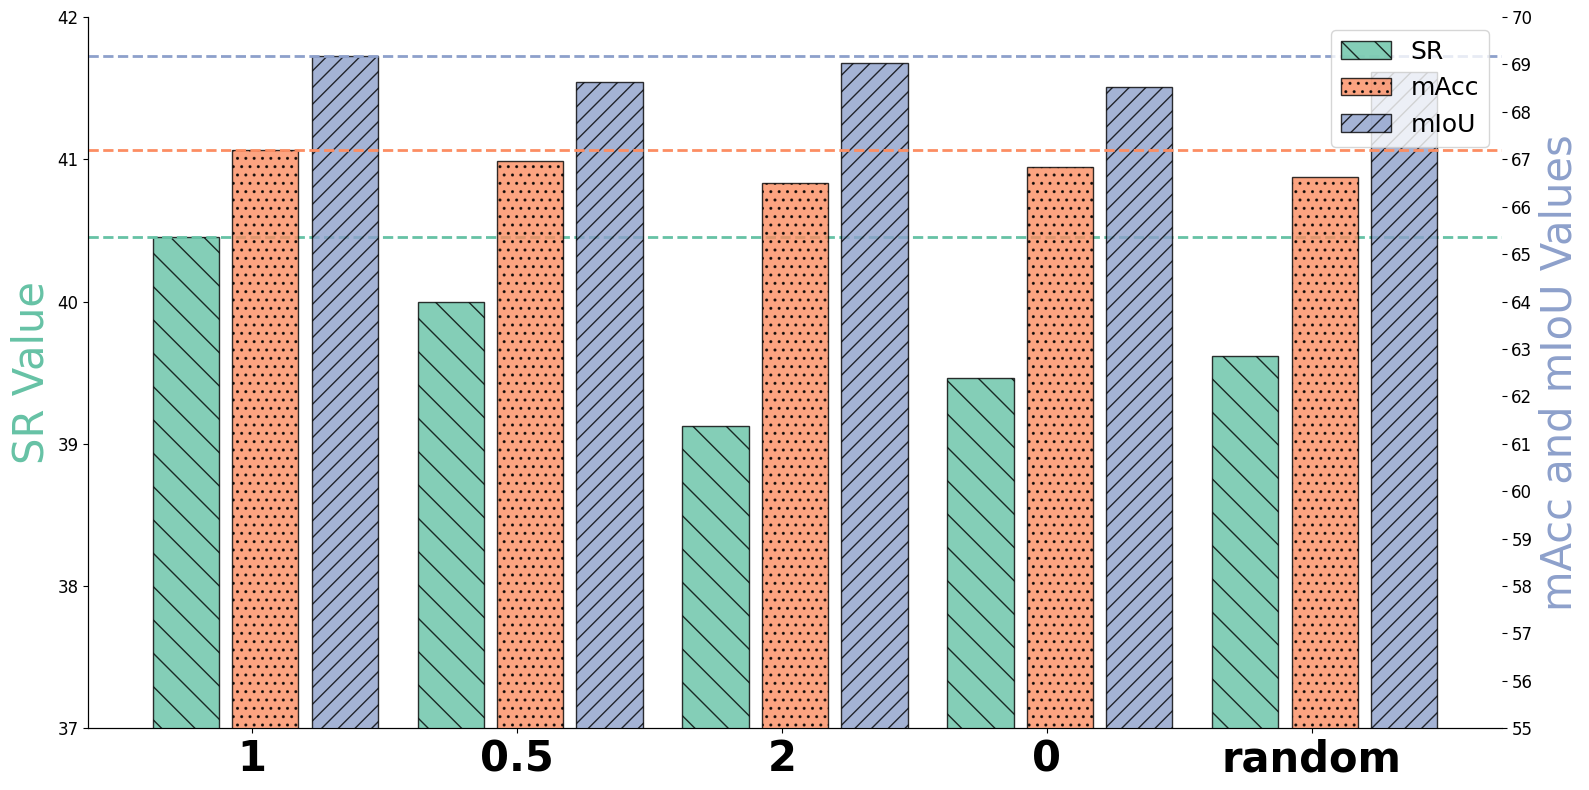
\includegraphics[width=0.45\textwidth]{figures/int1.png}
    \label{fig:int1}
}
\hfill
\subfloat[Ablation studies on different return values.]{%
    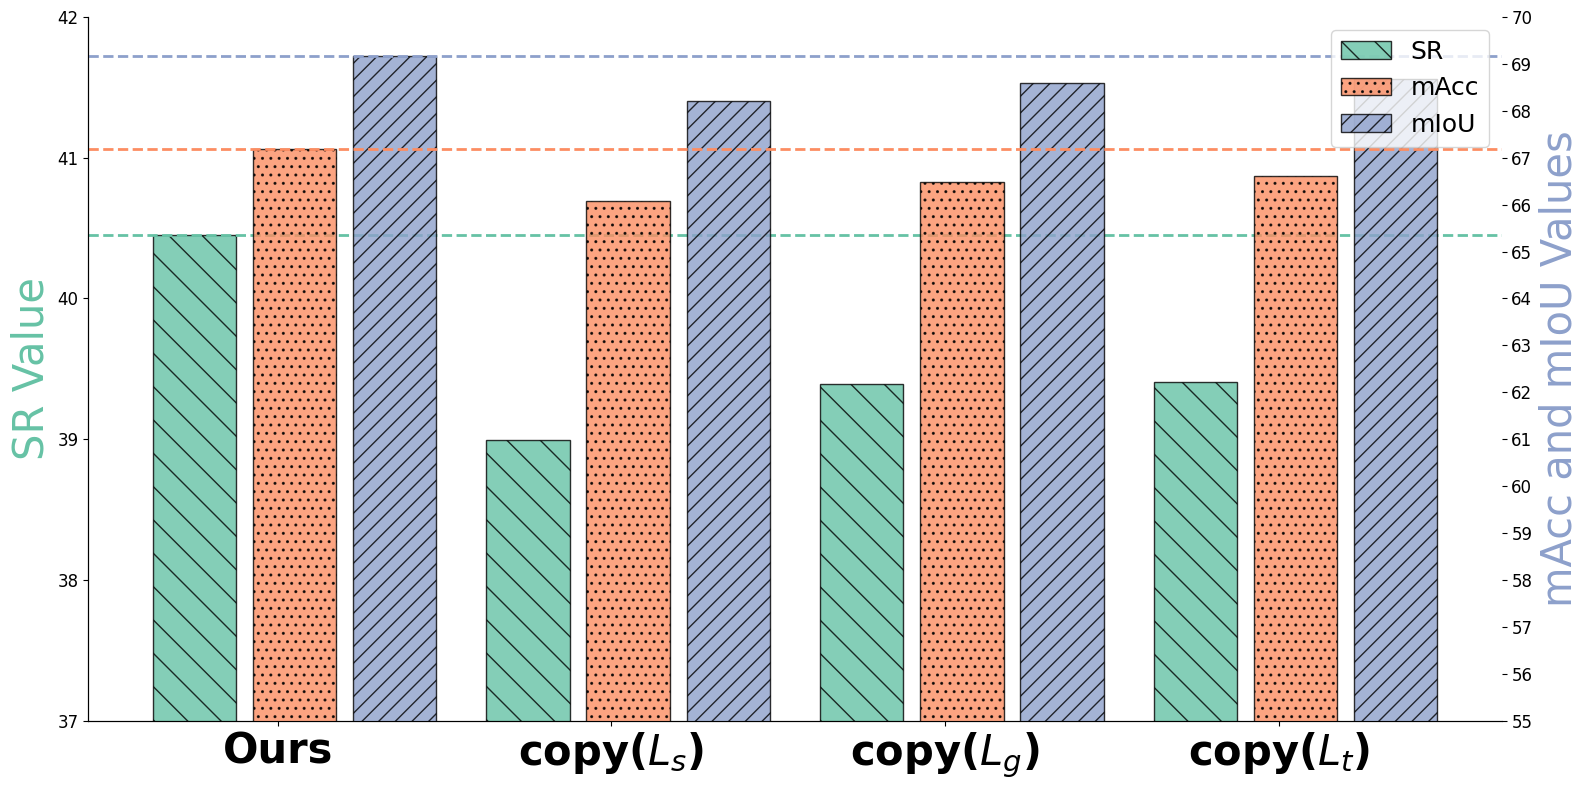
\includegraphics[width=0.45\textwidth]{figures/int2.png}
    \label{fig:int2}
}
\vfill
\subfloat[Ablation studies on selection with different interpolated features.]{
    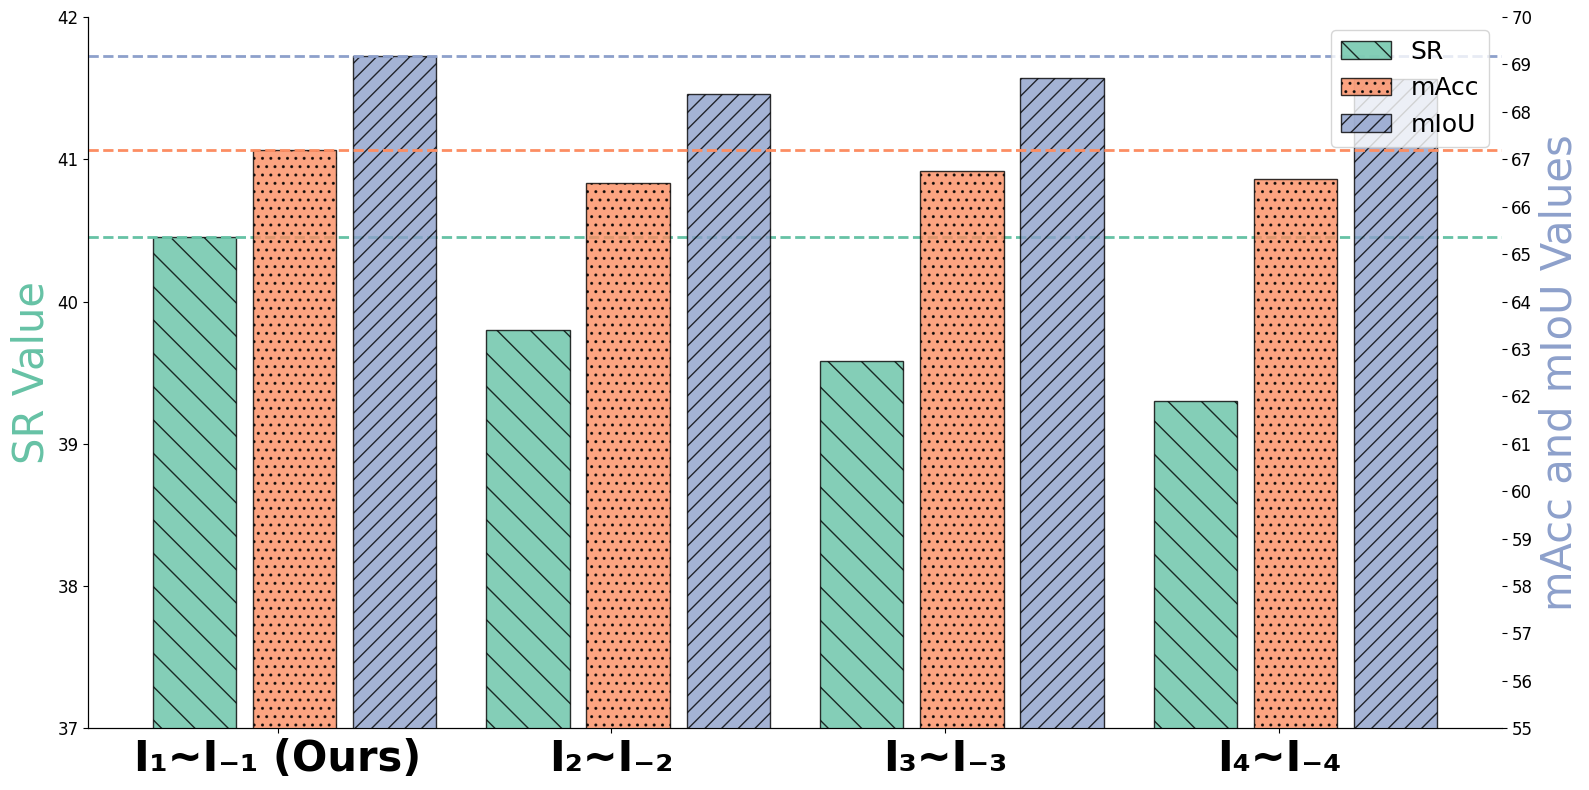
\includegraphics[width=0.45\textwidth]{figures/int3.png}
    \label{fig:int3}
}
\hfill
\subfloat[Ablation studies on different fusion methods.]{%
    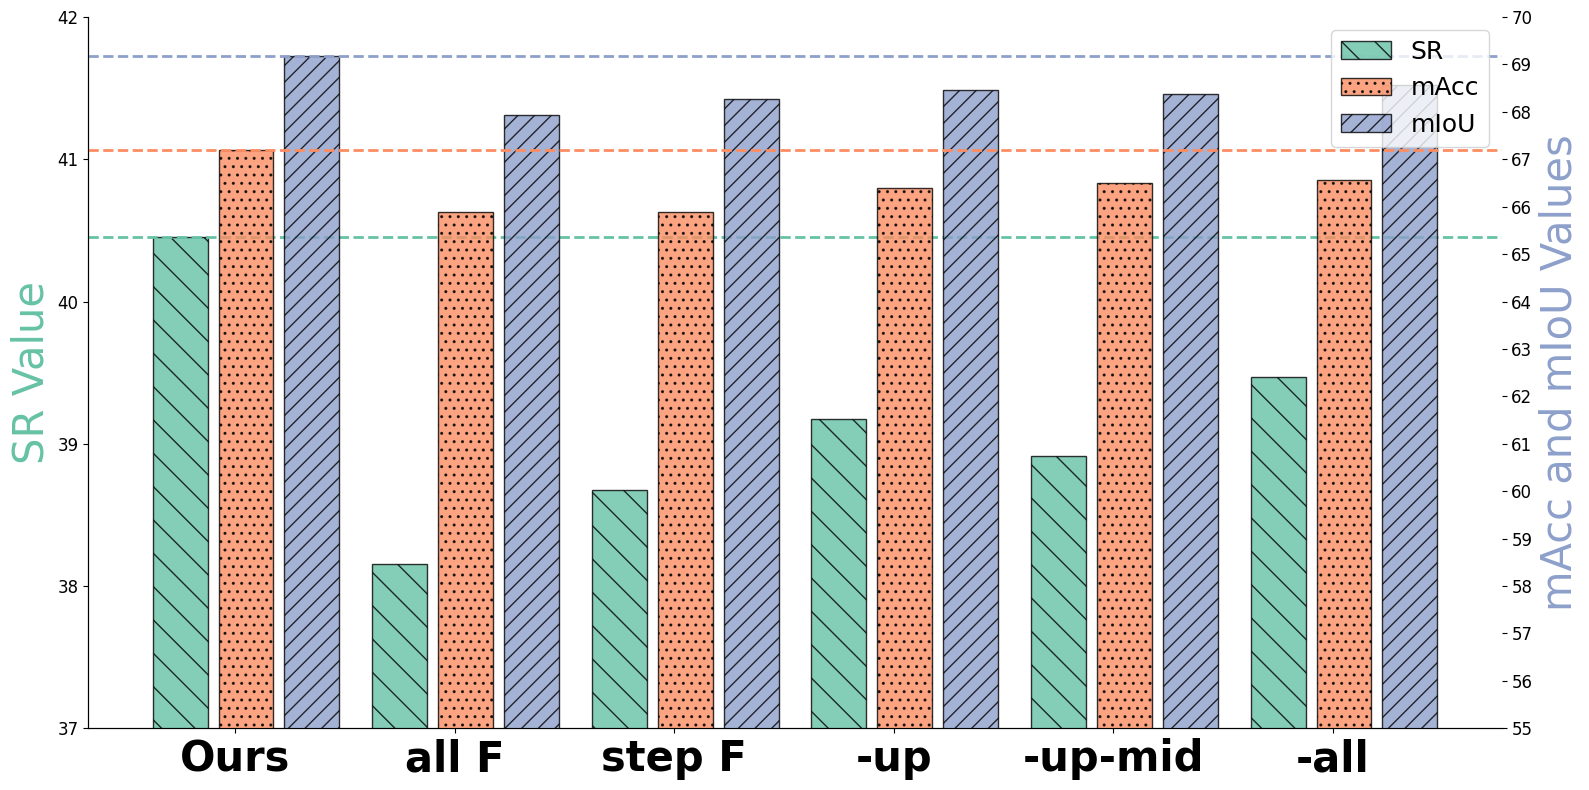
\includegraphics[width=0.45\textwidth]{figures/int4.png}
    \label{fig:int4}
}
\caption{Ablation Studies for Interpolation Strategy. \Cref{fig:int1} shows different initialization coefficient values $\tau$; \Cref{fig:int2} illustrates the features generated by the interpolator, where ``$copy(L_g)$'' means $I_j = L_g$, and ``$copy(L_t)$'' indicates $I_j = L_s$ for $j \leq \frac{M}{2}$ and $I_j = L_g$ for $j > \frac{M}{2}$. In \Cref{fig:int3}, $I_i$ to $I_{-i}$ indicates that we use interpolated features from the $i$-th to the last $i$-th for the second interpolation. In \Cref{fig:int4}, ``all F'' denotes that each cross-attention module receives $F_{1:M}$ as input, ``step F'' means we input one $F_{\frac{M}{2}}$ at the start and gradually increase the number of features inputted towards both sides, and ``-all'' indicates that we omit inputting $F_j$ during the upsampling, middle-sampling, and downsampling processes in U-Net. }
\label{fig:four_images2}
\end{figure}




% 加上ablation for 100%的结果,展示出分类器仍有不足。





% Following \citet{wang2023pdpp}, we enhance the diffusion model by incorporating a mask during the noise generation process, focusing on the $CrossTask_{How}$ dataset due to its high planning uncertainty.

\begin{wraptable}{r}{0.55\textwidth}
\vspace{-10pt}
\centering
\caption{Component ablation. Note: Int: Interpolation, Enc: Encoder, Trans: Transformer.}
\label{tab:component_ablation}
\scalebox{0.8}{
\begin{tabular}{@{}*{7}{>{\centering\arraybackslash}m{0.07\textwidth}}@{}}
\toprule
ID & Int & Enc & Trans & SR$\uparrow$ & mAcc$\uparrow$ & mIoU$\uparrow$ \\ 
\midrule
1 & \checkmark &  &  & 37.86 & 65.42 & 67.32 \\
2 & \checkmark & \checkmark &  & 39.23 & 66.62 & 68.44 \\
3 & \checkmark &  & \checkmark & \underline{39.49} & \underline{66.81} & \underline{68.68} \\
4 & \checkmark & \checkmark & \checkmark & \textbf{40.45} & \textbf{67.19} & \textbf{69.17} \\
\bottomrule
\end{tabular}
}
\vspace{-10pt}
\end{wraptable}
\textbf{Latent Space Temporal Logical Interpolation Module.} To evaluate the impact of various components within the module, we conduct ablation studies on the CrossTask dataset with $T=3$. \Cref{tab:component_ablation} presents the results. The findings indicate that the observation encoder effectively transforms visual observations into latent features, enhancing causal inference and capturing temporal logic. The interpolator enriches these features by generating multiple interpolated versions, which aids in reasoning. The transformer encoder further refines these features, ensuring both mathematical interpolation and logical consistency, thereby improving the model's inference capabilities.


\textbf{Interpolation Strategy.} \Cref{fig:four_images2} illustrates our adapted interpolation strategies for contrast. 
Initially, we test different initialization $\tau$ values in \Cref{fig:int1}. The highest score occurs when $\phi$ is initialized to 1, which proves to be the most stable and achieves the best overall performance, indicating that $\phi$ converges close to 1. 
Further experiments in \Cref{fig:int2} compare the use of $L_s$, $L_g$, or a combination of both through copying and direct return. The results show that directly returning $L_g$ performs well, suggesting that $V_g$ may play a critical role in action sequence inference. Although $L_s$ and $L_g$ are unadjusted features, the transformer encoder blocks can refine them to capture richer temporal logic and filter out irrelevant details, resulting in relatively reasonable scores. 
Additionally, we perform a second interpolation using the obtained $F_j$ (\Cref{fig:int3}). This experiment shows that as the features shift towards the center (from $F_i$ to $F_{-i}$), performance declines due to the loss of original information, aligning with our intuition. 
In \Cref{fig:int4}, we examine different fusion strategies for cross-attention. The ``all F'' approach results in sub-optimal performance, potentially due to the inclusion of numerous features being limited by the capacity of the layers, which diminishes the amount of information each feature can carry and introduces disorder. Similarly, the ``step F'' strategy may suffer from the same issue. When cross-attention is removed from various stages of the U-Net, we observe that the more layers are removed, the worse the results become. However, when all layers are removed, the results improve slightly, suggesting that introducing latent features into the U-Net without sufficient information disturbs the original distribution, leading to sub-optimal outcomes.



\subsection{Uncertainty Modeling} 
We present the uncertainty modeling results for CrossTask and NIV in \Cref{tab:combined_uncertainxx}. Two baselines from \citet{wang2023pdpp} are used for comparison: the $Noise$ baseline, which samples from random noise and uses the given observations and task class condition to obtain results in a single step without the diffusion process, and the $Deterministic$ baseline, where $\hat{x}_N=0$ and the model predicts a fixed outcome. We evaluate performance using $KL$ $divergence$, $NLL$, $ModeRec$, and $ModePrec$, as outlined in \citet{zhao2022p3iv}.

Our approach outperforms the baselines on CrossTask, particularly in modeling uncertainty and generating diverse plans. Compared to \citet{wang2023pdpp}, our model excels in the deterministic setting with $T=3$, demonstrating its ability to capture latent temporal relationships even with fewer time steps. For the NIV dataset, we observe that despite its small size, our diffusion-based process still delivers improvements. Additional visualizations are provided in the appendix.


\begin{table}[htbp]
% \vspace{-4mm}
\centering
\caption{The results of uncertain modeling on the CrossTask and NIV datasets.}
\scalebox{0.92}{
\begin{tabular}{l l cccc c cc}
\toprule
& & \multicolumn{4}{c}{CrossTask} & & \multicolumn{2}{c}{NIV} \\
\cline{3-6} \cline{8-9}
Metric & Method & $T=3$ & $T=4$ & $T=5$ & $T=6$ & & $T=3$ & $T=4$ \\
\midrule
\multirow{3}*{KL-Div $\downarrow$}
& Deterministic & 3.12 & 3.88 & 4.39 & \underline{4.04} & & 5.40 & \bf 5.29 \\
& Noise & \underline{2.75} & \underline{3.16} & \underline{4.37} & 4.74 & & \underline{5.36} & 6.03 \\
& Ours & \bf 2.66 & \bf 2.81 & \bf 2.12 & \bf 1.97 & & \bf 4.65 & \underline{5.47} \\
\midrule
\multirow{3}*{NLL $\downarrow$}
& Deterministic & 3.70 & 4.45 & 4.98 & 5.34 & & 5.48 & \bf 5.42 \\
& Noise & \underline{3.33} & \underline{4.04} & \underline{4.95} & \underline{5.32} & & \underline{5.44} & 6.12 \\
& Ours & \bf 3.24 & \bf 3.69 & \bf 3.22 & \bf 3.27 & & \bf 4.74 & \underline{5.56} \\
\midrule
\multirow{3}*{ModePrec $\uparrow$}
& Deterministic & 52.76 & 41.13 & \underline{31.46} & 18.65 & & \underline{27.77} & 26.48 \\
& Noise & \underline{54.30} & \underline{46.15} & 22.52 & \underline{19.09} & & 23.19 & \underline{32.39} \\
& Ours & \bf 56.19 & \bf 47.05 & \bf 32.75 & \bf 22.98 & & \bf 30.75 & \bf 35.88 \\
\midrule
\multirow{3}*{ModeRec $\uparrow$}
& Deterministic & 31.71 & 20.55 & 18.70 & 4.63 & & 26.48 & 21.57 \\
& Noise & \underline{43.92} & \underline{22.35} & \underline{21.53} & \underline{17.53} & & \underline{32.39} & \underline{23.75} \\
& Ours & \bf 47.34 & \bf 37.97 & \bf 39.64 & \bf 35.03 & & \bf 35.88 & \bf 29.90 \\
\bottomrule
\end{tabular}
}
\label{tab:combined_uncertainxx}
\end{table}



\section{Conclusion}
In this work, we introduced MTID, a novel masked temporal interpolation diffusion model designed for procedure planning in instructional videos. Our approach employs an interpolating predictor within a U-Net architecture, leveraging start and end frame features to infer intermediate states. By integrating a masking strategy during inference and loss calculation, we ensure the accuracy of the generated action sequences. Extensive experiments across various datasets confirm our model's superior performance in key metrics. Future research directions include establishing a benchmark dataset specifically aimed at tracking state changes in instructional content and exploring the implications of state change tracking in other procedural learning tasks such as pre-training and future step forecasting. Moreover, the challenge of multimodal procedural planning, involving the coherent generation of textual and visual plans, represents a promising area for further investigation.

\subsubsection*{Acknowledgments}
Use unnumbered third level headings for the acknowledgments. All
acknowledgments, including those to funding agencies, go at the end of the paper.

This work is supported by U.S. DARPA KAIROS Program No. FA8750-19-2-1004. The views and conclusions contained herein are those of the authors and should not be interpreted as necessarily representing the official policies, either expressed or implied, of DARPA, or the U.S. Government. The U.S. Government is authorized to reproduce and distribute reprints for governmental purposes notwithstanding any copyright annotation therein.


\FloatBarrier
\bibliography{iclr2025_conference} % for arxiv
\bibliographystyle{iclr2025_conference}% for arxiv
\section*{Appendix}
\appendix
\section{IMPLEMENTATION DETAILS}
In Section \ref{method2}, we presented the framework of our MTID. Additional details on the implementation of the model, encompassing both its architecture and training procedures, are provided in the appendix.

\textbf{Details of model architecture.}Our state decoder and step decoder are Transformer-based models. The model consists of two blocks. Each block consists of one
self-attention module, one cross-attention module, and a two-layer projection module.The input
query is first processed by the self-attention module, then forwarded to the cross-attention module,
and processed by the projection module. The cross-attention module takes the external memory to
calculate the keys and values. Each self-attention and cross-attention module consists of 32 heads
and the hidden layer size is set as 128. The step classifier is a two-layer MLP with hidden size of 128.
The dropout ratio is 0.2.\textbf{need to reconfirm}

\textbf{Details of training.}We utilize a linear warm-up approach for training our model. The specific training protocols vary across different datasets due to their varying scales. For the \texttt{CrossTaskBase} dataset, the diffusion step is set to 200, and training is conducted over 12,000 steps. The learning rate is increased linearly to \(8 \times 10^{-4}\) during the first 4,000 steps and then reduced to \(4 \times 10^{-4}\) at step 10,000. For the \texttt{CrossTaskHow} dataset, we maintain a diffusion step of 200 and extend training to 24,000 steps. Here, the learning rate rises linearly to \(5 \times 10^{-4}\) over the first 4,000 steps, followed by a reduction by a factor of 0.5 at steps 10,000, 16,000, and 22,000. In the case of the \texttt{NIV} dataset, with a diffusion step of 50, we perform training for 6,500 steps due to its smaller size. The learning rate increases linearly to \(3 \times 10^{-4}\) over the initial 4,500 steps and then decays by 0.5 at step 6,000. For the \texttt{COIN} dataset, which requires more extensive training due to its large scale, we set the diffusion step to 200 and train for 160,000 steps. The learning rate is increased linearly to \(1 \times 10^{-5}\) within the first 4,000 steps, and then it is reduced by a factor of 0.5 at steps 14,000 and 24,000, with the rate remaining at \(2.5 \times 10^{-6}\) for the remaining steps. The batch size for all experiments is set to 256, and we use a weighted loss with \(w = 10\). All experiments are executed using ADAM \cite{23} on 8 NVIDIA RTX 3090 GPUs.

\section{Baseline Methods}
In this section, we describe the baseline methods employed in our study.
\begin{itemize}
    \item \textbf{Random Selection.} This strategy involves randomly choosing actions from the available action space within the dataset to generate plans.
    \item \textbf{Retrieval-Based Approach.} For the given observations \(\{os, og \}\), this method retrieves the closest matching neighbor by evaluating the minimum visual feature distance in the training dataset. The action sequence associated with the retrieved neighbor is then used as the plan.
    \item \textbf{WLT DO \cite{10}.} This method utilizes a recurrent neural network (RNN) to forecast action steps based on the provided pairs of observations.
    \item \textbf{UAAA \cite{11}.} The UAAA technique is a two-stage process that leverages an RNN-HMM model to predict action steps in an autoregressive manner.
    \item \textbf{UPN \cite{33}.} UPN is a path planning algorithm for physical environments that learns a plannable representation to generate predictions. To derive discrete action steps, a softmax layer is appended to the model's output as described in \cite{4}.
    \item \textbf{DDN \cite{4}.} The DDN model is an autoregressive framework with two branches, designed to learn an abstract representation of action steps and predict transitions in the feature space.
    \item \textbf{PlaTe \cite{34}.} The PlaTe model extends DDN by incorporating transformer modules in its two branches for prediction tasks. It is important to note that PlaTe's evaluation protocol differs from other models, so comparisons with PlaTe are included in the supplementary material.
    \item \textbf{Ext-GAIL \cite{2}.} Ext-GAIL addresses procedure planning using reinforcement learning methods. Unlike our approach, Ext-GAIL splits the planning problem into two stages where the first stage provides long-horizon information for the second, whereas our goal is to derive sampling conditions.
    \item \textbf{P3IV \cite{42}.} The P3IV model is a transformer-based single-branch approach that includes a learnable memory bank and an additional generative adversarial framework. Similar to our model, P3IV forecasts all action steps simultaneously during the inference phase.
\end{itemize}

\textbf{State Descriptions.}need to add the details

\textbf{Results on COIN.}
Table~\ref{tab:niv} presents the outcomes on the COIN dataset. Consistent with the findings from CrossTask and COIN, our MTID method demonstrates superior SR and mIoU scores and maintains competitive mAcc performance.
We extract step sequences $a_{t:(t+T-1)}$ from the videos, where the horizon $T$ ranges from 3 to 6. Following~\citep{zhao2022p3iv,wang2023pdpp}, we generate action sequences $\{[a_i, ..., a_{i+T-1}]\}_{i=1}^{n-T+1}$ by sliding a window of size $T$ over the $n$ actions. For each sequence, the video clip feature at the start of action $a_i$ is used as the start observation $o_s$, and the feature at the end of $a_{i+T-1}$ as the goal state $o_g$, with both clips lasting 3 seconds.

Previous works~\citep{chang2020procedure, bi2021procedure, sun2022plate} computed the mIoU metric over mini-batches, averaging the results across the batch size. However, this method introduces variability based on the batch size. For example, if the batch size is set to the size of the entire dataset, all predicted actions may be deemed correct. In contrast, using a batch size of one penalizes any mismatch between predicted and ground-truth sequences. To address this issue, we follow \citet{wang2023pdpp} by standardizing mIoU calculation, computing it for each individual sequence and then averaging the results, which effectively treats the batch size as one.
\begin{table}[ht]
\centering
\begin{minipage}{\textwidth}
\centering
\caption{Comparisons on the NIV dataset.}
\scalebox{0.92}{
\begin{tabular}{l ccc c ccc}
\toprule
& \multicolumn{3}{c}{$T$ = 3} & & \multicolumn{3}{c}{$T$ = 4} \\ 
\cline{2-4} \cline{6-8}
{Models}           & SR$\uparrow$    & mAcc$\uparrow$   & mIoU$\uparrow$  &   & SR$\uparrow$    & mAcc$\uparrow$   & mIoU$\uparrow$ \\ \midrule
Random       &   2.21    &    4.07    &    6.09    &  &   1.12    &    2.73    &    5.84    \\
{DDN}              &   18.41    &    32.54    &    56.56    &  &   15.97    &    27.09    &    53.84    \\
{Ext-GAIL}              &   22.11    &    42.20    &    65.93    &  &   19.91    &    36.31    &    53.84    \\
{P$^3$IV}             &   24.68    &   49.01    &   74.29   &    &   20.14    &   38.36     &   67.29   \\
{EGPP} &   26.05    &   \bf 51.24   &   75.81   &   &   21.37    &  \bf 41.96     &   74.90  \\
\hline
{SCHEMA (Ours)} & \bf 27.93 & 41.64 & \bf 76.77 & & \bf 23.26 & 39.93 & \bf 76.75 \\
\bottomrule
\end{tabular}
}
\label{tab:niv}
\end{minipage}

\vspace{0.5cm}

\begin{minipage}{\textwidth}
\centering
\caption{The results of uncertain modeling on the CrossTask dataset.}%
\scalebox{0.92}{
\begin{tabular}{l l c c c c}
\toprule %
Metric & Method & $T=3$ & $T=4$ & $T=5$ & $T=6$ \\ %
\midrule %
\multirow{2}*{KL-Div $\downarrow$}
&  Ours - deterministic & 4.03 & 4.31 & 4.49 & 4.65 \\ %
&  Ours - probabilistic & \bf 3.62 & \bf 3.82 & \bf 3.92 & \bf 3.97 \\ %
\midrule %
\multirow{2}*{NLL $\downarrow$}
&  Ours - deterministic & 4.55 & 5.11 & 5.46 & 5.71 \\ %
&  Ours - probabilistic & \bf 4.15 & \bf 4.62 & \bf 4.88 & \bf 5.04 \\ 
\midrule %
\multirow{2}*{ModePrec $\uparrow$}
&  Ours - deterministic & \bf 38.41 & \bf 26.67 & \bf 15.28 & 9.84 \\ %
&  Ours - probabilistic & 38.32 & 26.46 & 14.99 & \bf 9.91 \\
\midrule %
\multirow{2}*{ModeRec $\uparrow$}
&  Ours - deterministic & 25.59 & 13.63 & 6.27 & 3.37
 \\ %
&  Ours - probabilistic & \bf 37.70 & \bf 23.76 & \bf 13.85 & \bf 9.30 \\
\bottomrule %
\end{tabular}
}
\label{tab:unc}
\end{minipage}

\end{table}


\section{Further Discussions}
This section offers further discussion on related works and presents insights that were excluded from the main paper due to space limitations.

\textbf{Limitations.}The limitations of our method are as follows. First, While the logic between the actions generated by our model is robust, there is still no guarantee of perfect alignment between the generated actions and the task. Instances of mismatches between them were observed in the experiments. This is a general challenge for procedure planning models, as The labels for multi-tasking and multi-action in the dataset are replaced by data ids,which will cause Problems with numerical calculations.To solve this challenge,we have tried to add the restriction of a masking mechanism to the iterative process, but it was ineffective due to interfering with the diffuse noise.Considering of the perfect performance of LLM,we tried to ues LLM to guide the process of generating actions,but the efficient of generation still falls short of our expectations.During our experiments, we found a way to add cross attention to U-Net at the same time and get a good results, but this method consumes a lot of resources, so we didn't use it.Secondly, our masking mechanism is not yet fully refined, leading to suboptimal performance on large-scale datasets. Further improvements are needed to enhance its effectiveness in handling more extensive and complex data. We will investigate further possibilities for applying Large Language Models (LLMs) to guide action generation and explore the use of generative Vision-Language Models (VLMs) for state description generation.

\textbf{Differences from other mid-state prediction methods.} Our approach differs from existing mid-state prediction methods in several key ways: (1) \textit{Compared to PDPP and Skip-Plan:} PDPP uses task labeling to eliminate the need for costly intermediate supervision, while Skip-Plan reduces prediction uncertainty by bypassing intermediate state supervision and breaking down long sequences. However, both methods struggle to effectively capture and represent mid-state information. To address this, we introduce a novel supervision mechanism that leverages latent temporal and logical features to better handle the mid-state process. (2) \textit{Compared to PlaTe and Ext-GAIL:} PlaTe and Ext-GAIL operate under a fully supervised setting, whereas our method works in a weak supervision setting, significantly reducing the need for detailed annotations. (3) \textit{Compared to methods under weak supervision:} Recent approaches like SCHEMA also consider weak supervision and annotate mid-states. However, SCHEMA focuses more on tracking and representing state changes, treating the process holistically without the need for labeling each intermediate state. In contrast, our method introduces explicit mid-state supervision for the first time and has achieved strong results, demonstrating the effectiveness of our approach.

\textbf{Comparisons with related works.}%还没决定要不要写这一部分,SCHE的这一部分是做的跟他相似工作的一个比较,但是你这个emmmmm,感觉找不到那么相关的工作,还在纠结

\textbf{Generalization capabilities.} Our method effectively addresses variations in action steps, object states, and environmental conditions. For action step variations, we tested the method with steps of different lengths, ranging from 3 to 6. The experimental results showed that our approach consistently surpassed state-of-the-art models. In terms of object states and environmental contexts, the benchmark datasets used for evaluation span a wide range of topics and domains, such as cooking, housework, and car maintenance, as well as diverse objects like fruits, drinks, and household items. For example, the CrossTask dataset includes 133 types of steps across 18 tasks, while the COIN dataset features 778 step types over 180 tasks. Testing on these datasets highlights the model's ability to generalize across varying object states and environmental conditions.

\end{document}
